\documentclass[12pt,a4paper]{article}
\usepackage[utf8]{inputenc}
\usepackage[francais]{babel}
\usepackage[T1]{fontenc}
\usepackage{amsmath}
\usepackage{amsfonts}
\usepackage{amssymb}
\usepackage{geometry}
\usepackage{enumitem}
\usepackage{hyperref}
\usepackage{graphicx}
\geometry{hmargin=3.0cm,vmargin=1.5cm}
\parindent=0pt

\title{Manuel Utilisateur}
\author{Auteur : Nicolas \bsc{REYNAUD}}
\date{8 janvier 2015}

	
\begin{document}
%--------------------------Page de présentation------------------------------%
\maketitle

\newpage

\section{Introduction}

Dans ce document nous verrons comment utiliser les outils de la team KNK.\\

Nous verrons alors l'utilisation du client et du serveur.

\section{Lancement}

Pour lancer le serveur ou le client, commencer par double cliquer sur les icônes associés.
A noter : Vous DEVEZ lancer le serveur avant de lancer le client.

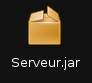
\includegraphics[scale=0.6]{images/serveur.png} 

\includegraphics[scale=0.7]{images/client.png}

Après avoir double cliqué sur les icones du programme les fenêtres suivantes apparaitrons. 

\begin{center}

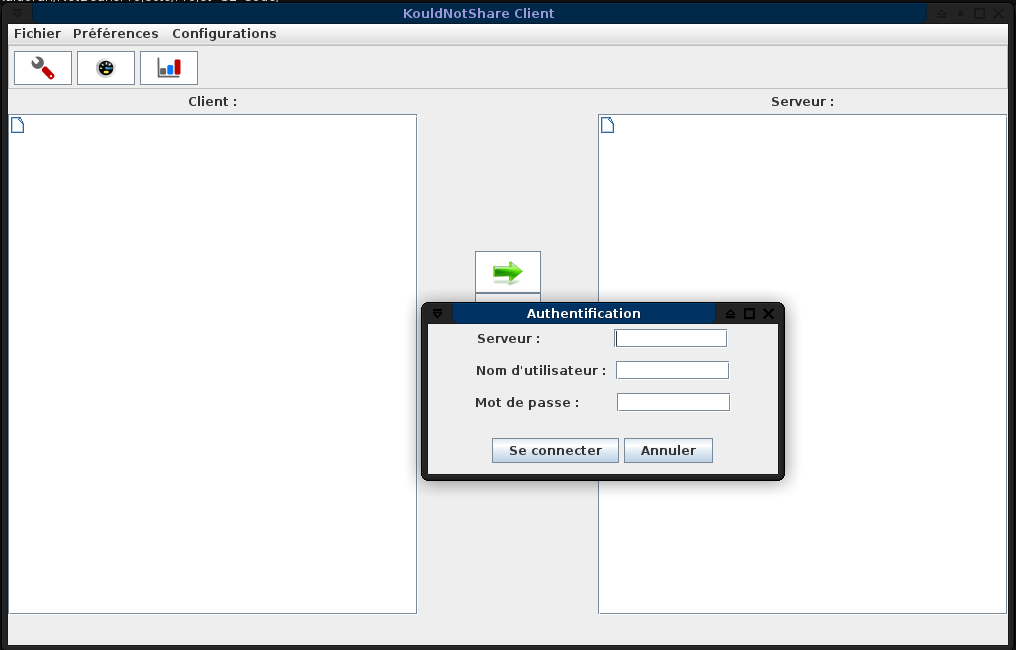
\includegraphics[scale=0.3]{images/clientlance.png} \\
Le client une fois lancé

\end{center}

\begin{center}
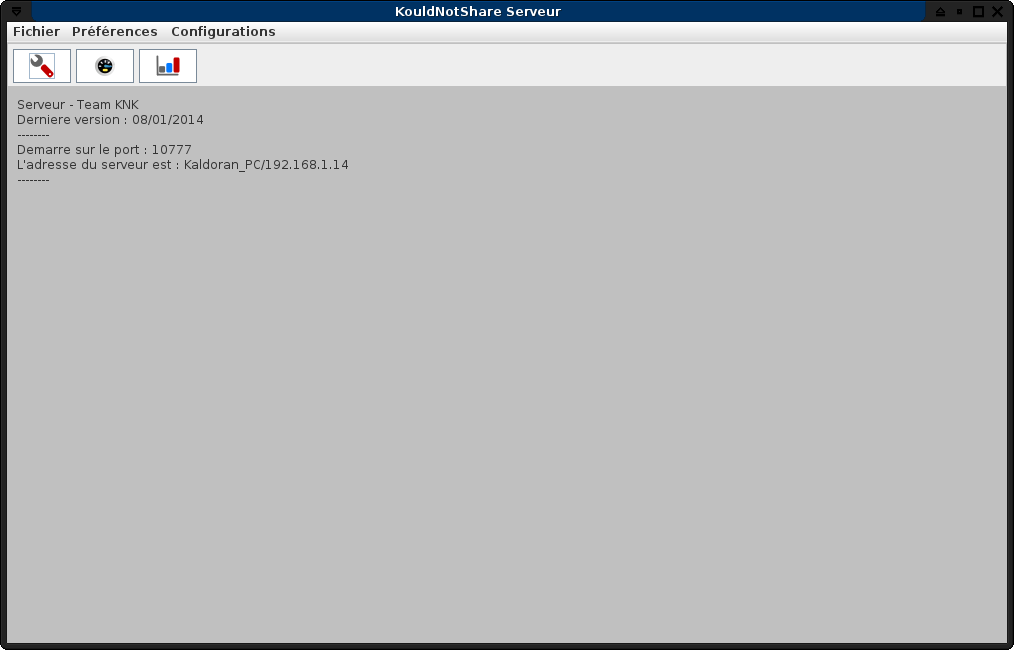
\includegraphics[scale=0.3]{images/serveurlance.png} \\
Le serveur une fois lancé
\end{center}

Nous allons maintenant détailler le principe de fonctionnement du client. \\
La version du serveur n'étant qu'a un stade primaire, celui ci est fournit dans le seul but de tester le client. \\

\newpage
\section{Principe de fonctionnement du client}

Dès l'ouverture du programme "Client" un pop-up d'authentification apparait.

\begin{center}
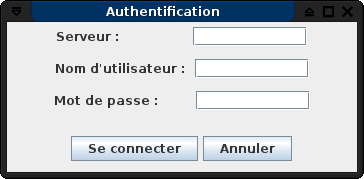
\includegraphics[scale=0.5]{images/clientlancelogin.png}
\end{center}

Il vous faudra alors compléter les champs pour vous authentifier.

\underline{A noter} : Si le serveur est en locale ( sur votre propre machine ). \\
l'adresse du serveur sera alors : \textbf{127.0.0.1} \\

Le nom d'utilisateur et le mot de passe vous seront fourni par le responsable du serveur.

\underline{A noter} : Le serveur est fourni de base avec 3 comptes : \\
\begin{itemize}
	\item Compte 1
		\subitem Pseudo : Kaldoran 
		\subitem Mot de passe : 123456 
	\item Compte 2
		\subitem Pseudo : baba
		\subitem Mot de passe : 123456
	\item Compte 3
		\subitem Pseudo : lala
		\subitem Mot de passe : 123456
\end{itemize}

Il est de la responsabilité du responsable du serveur de supprimer ses comptes. \\

Après avoir cliqué sur le bouton "Se connecter" des erreurs peuvent apparaitre. \\
Si tel est le cas se référer a la section "Les Cas d'erreur". \\

Dans le cas contraire, le pop-up disparait. \\
Félicitation vous êtes maintenant connecté. \\

Si vous cliquez sur annulé, vous aurez alors accès aux options mais pas aux fichier du serveur.
\subsection{Les cas d'erreur}

Plusieurs cas d'erreur / message d'erreurs peuvent apparaitre. \\

\begin{center}

	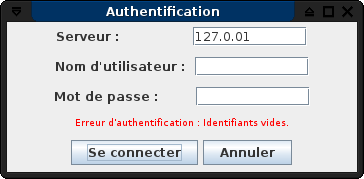
\includegraphics[scale=0.5]{images/erreurvide.png} \\
	Si ceci apparait, vous avez oublier de remplir UN ou PLUSIEURS champs. \\

	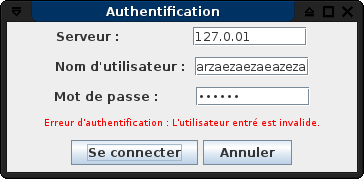
\includegraphics[scale=0.5]{images/erreurpseudo.png} \\
	Cette erreur apparait si votre pseudo est trop long. \\

	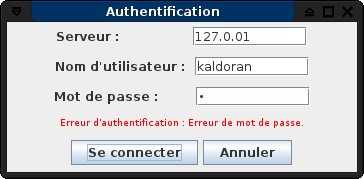
\includegraphics[scale=0.5]{images/erreurpass.png} \\
	Cette erreur apparait si votre mot de passe est trop court / trop long. \\

	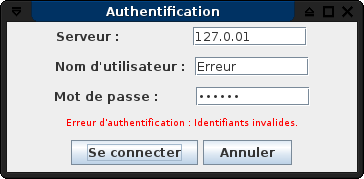
\includegraphics[scale=0.5]{images/erreurid.png} \\
	Cette erreur se produit si le compte entré n'existe pas sur le serveur. \\

\end{center}

\subsection{Visuel}
Une fois le pop-up disparue, une fenêtre de ce type devrait apparaitre.

\begin{center}
	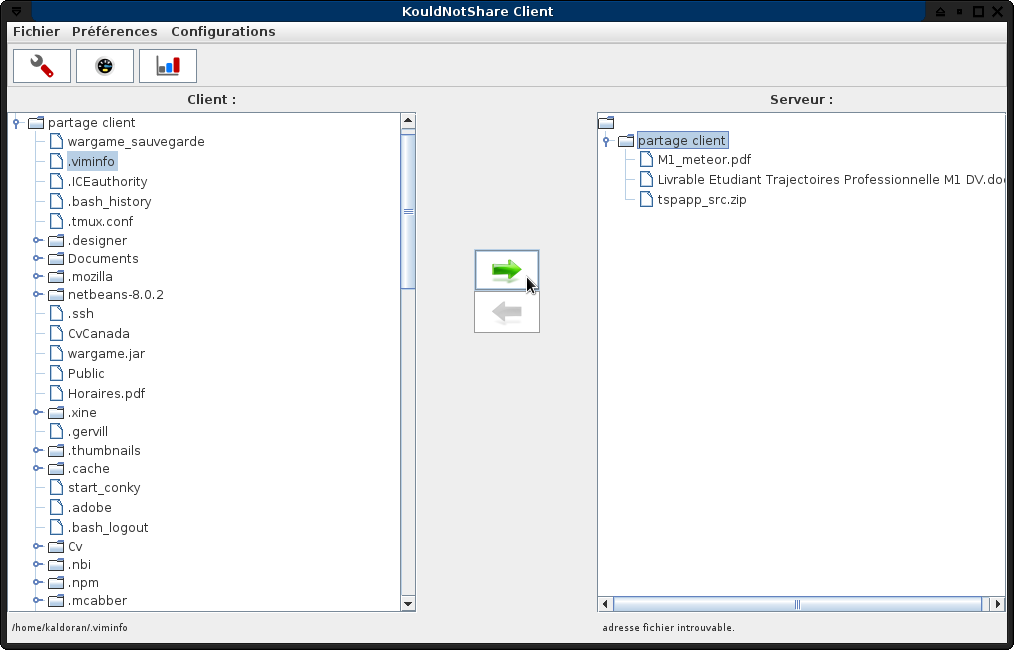
\includegraphics[scale=0.4]{images/envoi.png} \\
	En haut se trouve la barre des menus. \\
	Juste en dessous la barre des options. \\
	
	Pour finir la fenêtre se divise en 2 parties. \\
	A droite : Les fichiers provenant du serveur. \\
	A gauche : Les fichiers présent sur votre ordinateur. \\
	
	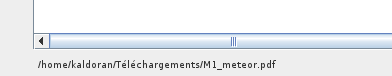
\includegraphics[scale=0.4]{images/chemin.png} \\
	Vous pourrez également remarquer sur le screen que en dessous de chaque coté le chemin du fichier sélectionné est indiqué.

\end{center}


\subsection{Visualisation des fichiers}
\begin{center}
	Par défaut les répertoires sont replié. Un simple double clique les ouvrira. \\
	Passant alors de ceci : \\
	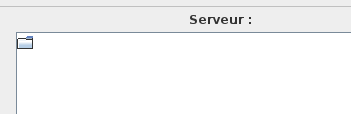
\includegraphics[scale=0.5]{images/fichier.png} \\

	A ceci : \\
	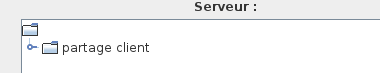
\includegraphics[scale=0.5]{images/dev.png} \\
	
	Vous pourrez des lors cliquer sur les icônes bleu pour développer les fichier, ou double cliquer sur les fichier pour les ouvrir.
	
\end{center}

\subsection{Envoi de fichier}

\begin{center}
	Pour réaliser l'envoi d'un fichier sur le serveur, vous devez sélectionner  votre fichier dans la partie gauche du logiciel. \\
	Les fichiers sont symbolisé par des petites feuilles blanches. \\
	Puis ensuite sélectionner le dossier dans la partie droite dans lequel vous souhaitez envoyer le fichier. \\
	Pour finir cliquez sur la flèche allant vers la droite. \\
	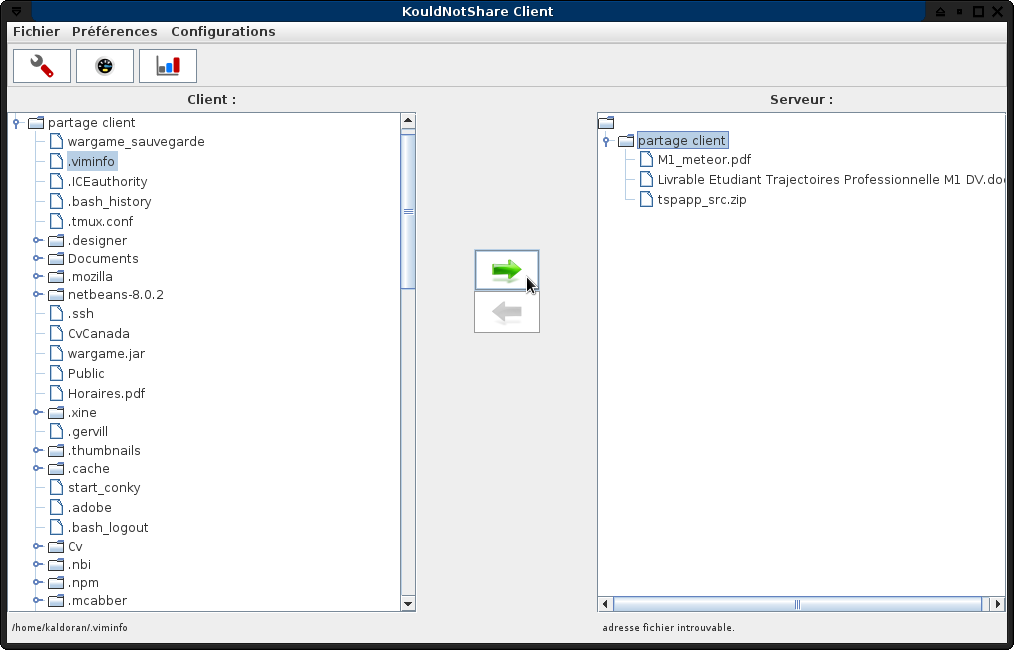
\includegraphics[scale=0.4]{images/envoi.png}
	Un résumé de la procédure, ici le fichier '.viminfo' sera transféré dans le dossier : 'Partage client'. 

\end{center}

\subsection{Récupération de fichier}

\begin{center}
	Pour récupérer un fichier commencez par sélectionner le fichier dans la partie droite du programme. \\
	Puis sélectionnez un répertoire dans la partie gauche du programme. \\
	Cliquez ensuite sur la flèche orientée vers la gauche. \\
	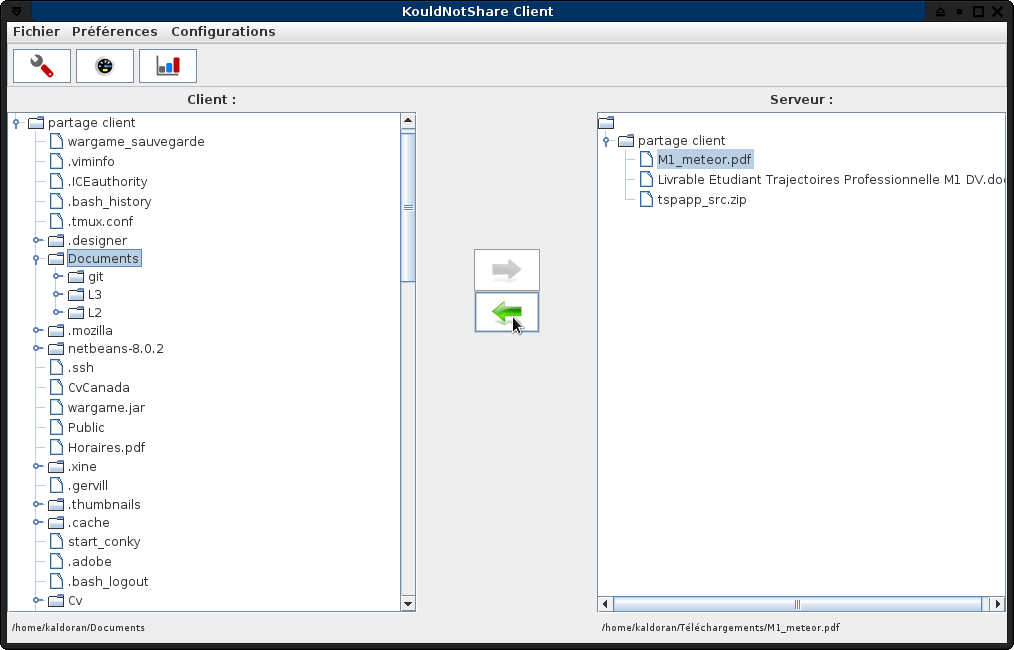
\includegraphics[scale=0.4]{images/get.png} \\
	Un résumé de la procédure. Ici le fichier 'M1\_meteor.pdf' sera transféré dans le dossier 'Documents'. 
\end{center}


\subsection{La barre des menus}
\begin{center}
	
\includegraphics[scale=0.5]{images/menu.png} \\
	Cette barre a été désactivée.
\end{center}

\subsection{Les options de configuration}
\begin{center}
	
\includegraphics[scale=0.5]{images/option.png} \\
	Cette barre a été désactivée.
\end{center}
\end{document}